\documentclass[12pt]{article}
\usepackage{graphicx}
\author{Manuel González González}
\title{Práctica 7: Perceptrón multicapa Opcional}
\begin{document}
\maketitle

\section*{Ejercicio 2}
\subsection*{f)}
Estamos pidiendo que clasifique los patrones de entrada entre la clase 0 y la clase 1.

\subsection*{g)}
El mínimo alcanzado por Beta 1.0 es mejor que el de 0.1. Esto se debe a que la función que usamos para el ajuste se parece más al conjunto de datos objetivo.

\begin{figure}
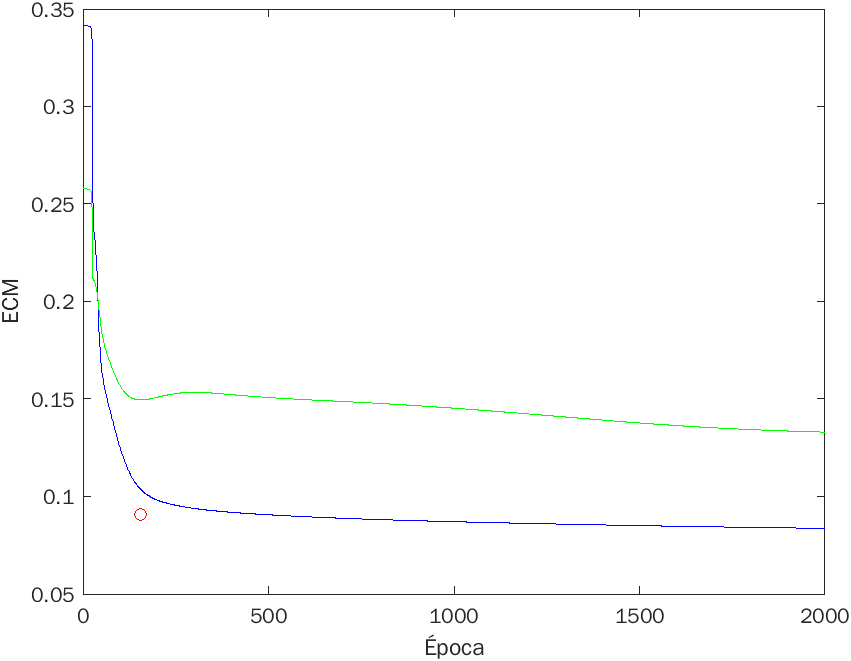
\includegraphics[scale=1]{2g1_1.png}
\caption{Primera ejecución con Beta 1.0}
\end{figure}
\begin{figure}
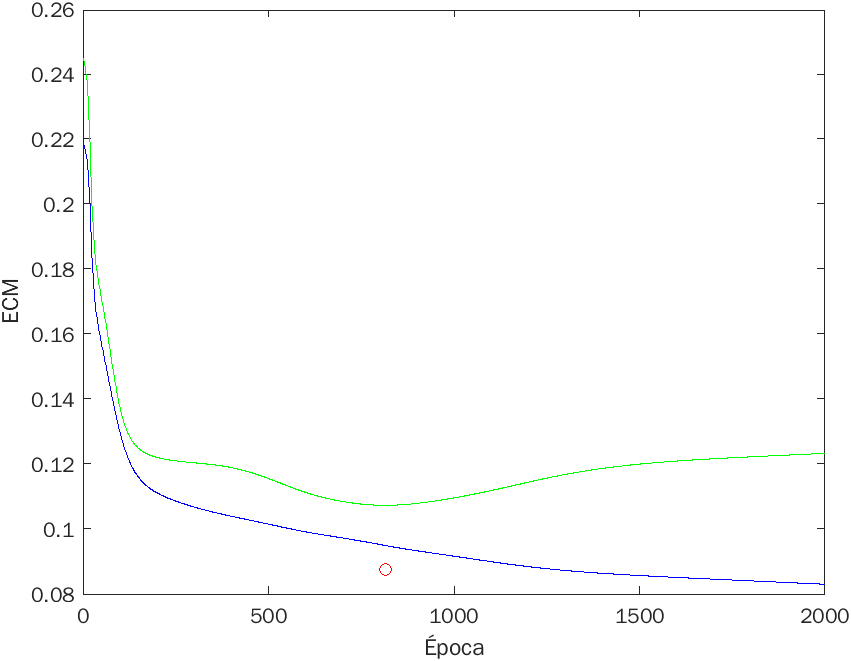
\includegraphics[scale=1]{2g2_1.png}
\caption{Segunda ejecución con Beta 1.0}
\end{figure}
\begin{figure}
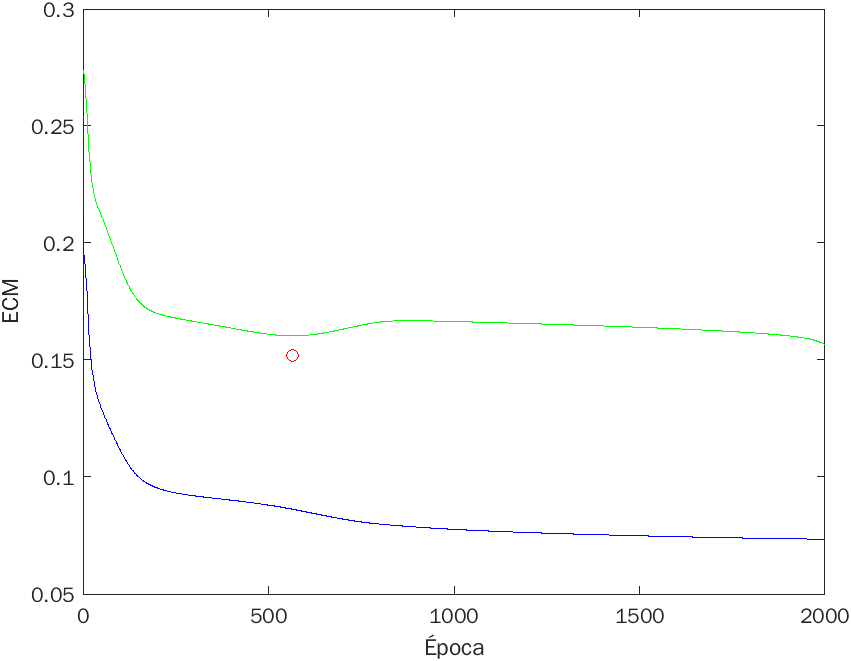
\includegraphics[scale=1]{2g3_1.png}
\caption{Tercera ejecución con Beta 1.0}
\end{figure}
\begin{figure}
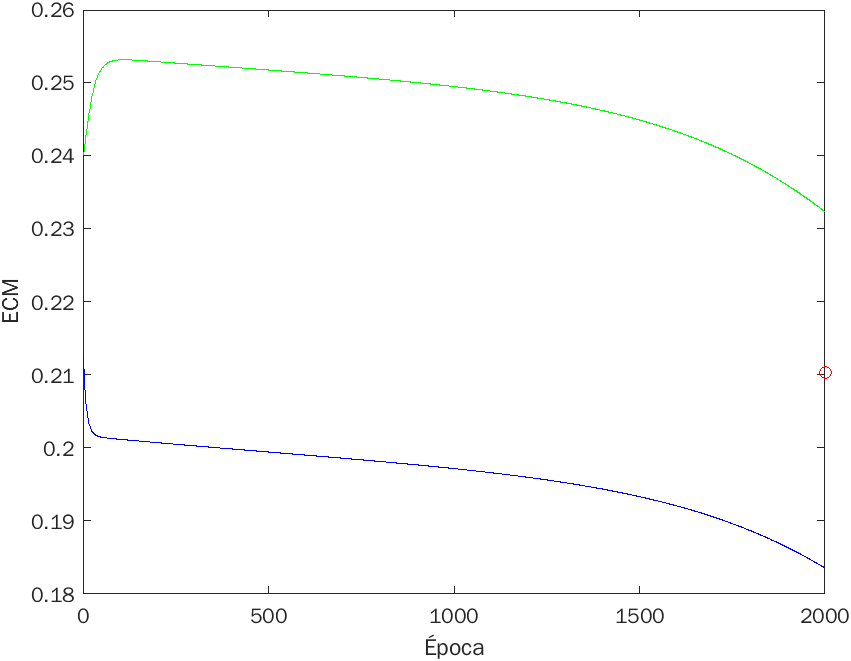
\includegraphics[scale=1]{2g1_01.png}
\caption{Primera ejecución con Beta 0.1}
\end{figure}
\begin{figure}
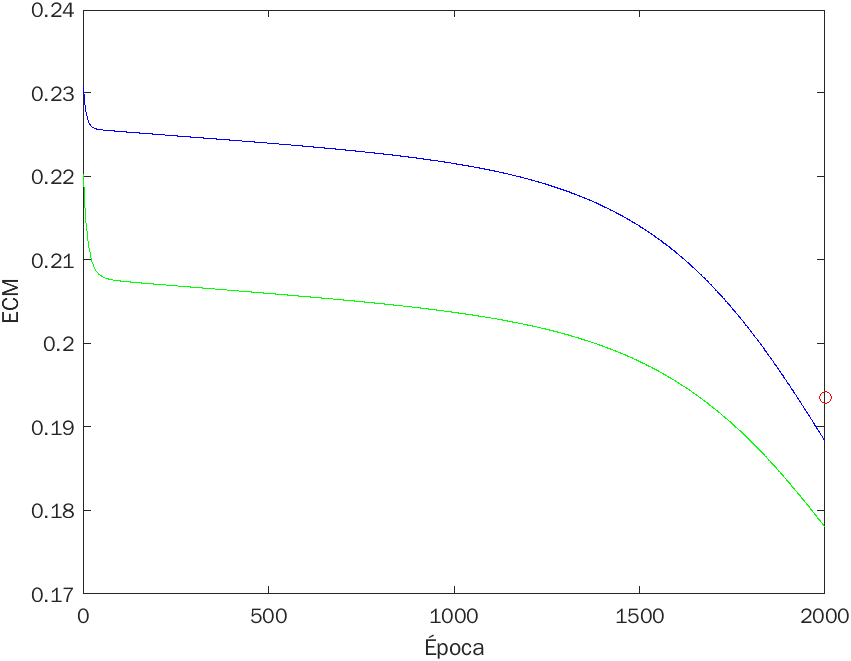
\includegraphics[scale=1]{2g2_01.png}
\caption{Segunda ejecución con Beta 0.1}
\end{figure}
\begin{figure}
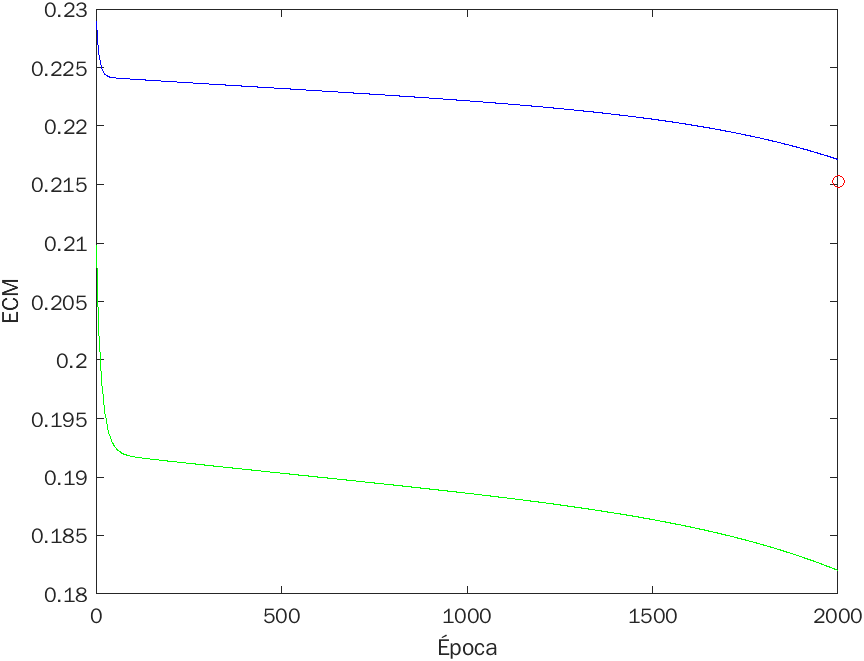
\includegraphics[scale=1]{2g3_01.png}
\caption{Tercera ejecución con Beta 0.1}
\end{figure}
\newpage
\section*{Ejercicio 3}
\subsection*{a)}
El rango es un intervalo entre 0 y 1.

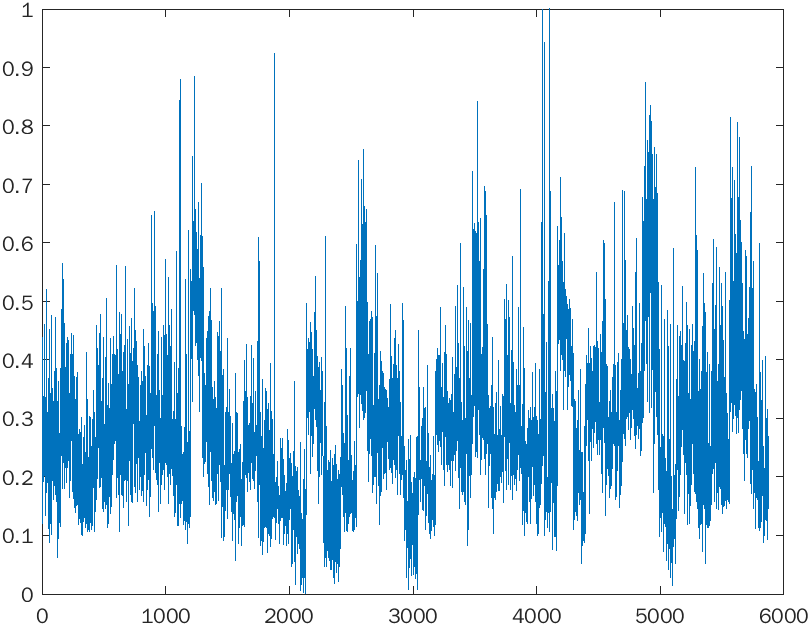
\includegraphics[scale=1]{3a.png}

\subsection*{b)}
Le estamos pidiendo que haga una regresión de una función general.

\subsection*{c)}
El mínimo con 1.0 es 0.537 y el mínimo con 0.1 es 0.005, es decir, es mejor con Beta 0.1. Esto se debe a que cuando es 1.0 la función se asemeja a la función escalón y el conjunto de datos objetivo no se ve representado por dicha función, ya que no se trata de una clasificación.

\begin{figure}
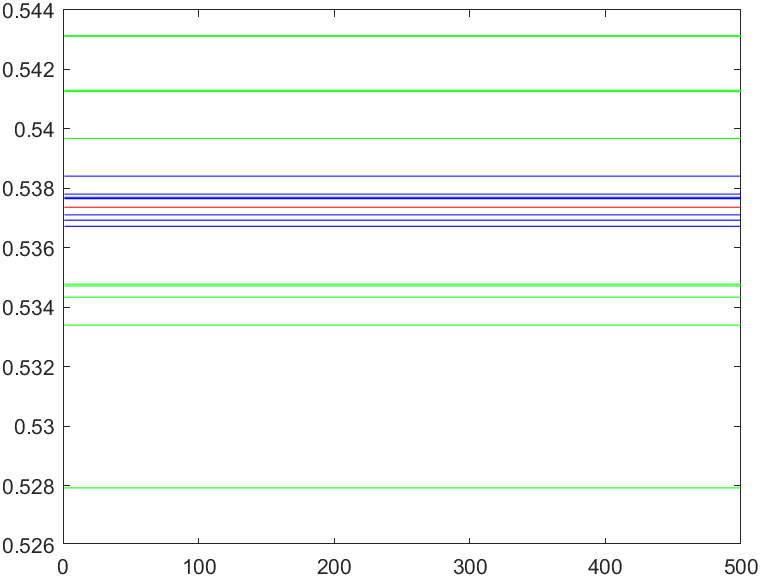
\includegraphics[scale=1]{3c_1.png}
\caption{Ejecución con Beta 1.0}
\end{figure}

\begin{figure}
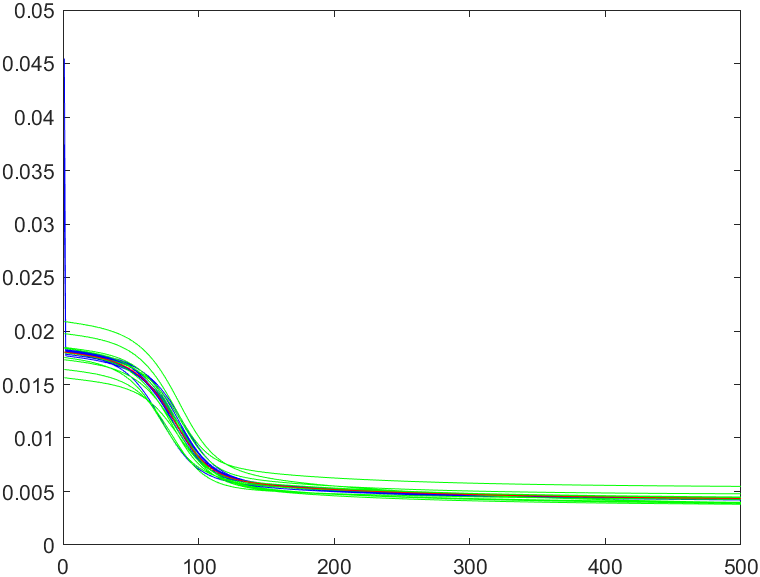
\includegraphics[scale=1]{3c_01.png}
\caption{Ejecución con Beta 0.1}
\end{figure}


\end{document}